\documentclass[12pt]{article}
\usepackage{graphicx}
\usepackage{fancyhdr}
\usepackage{varwidth}
\usepackage{commath}
\usepackage{xspace}
\usepackage{tikz}
\usepackage{gensymb}
\usepackage[margin=0.5in]{geometry}
\usepackage{amsmath}
\usepackage{mathtools}
\begin{document}
\begin{center}
\addtolength{\topmargin}{.25in}

\pagestyle{fancy}
\lhead{Steven Seiden}
\rhead{The ``Ultimate" Math Formula Sheet}

\fbox{\parbox{\dimexpr\linewidth-2\fboxsep-2\fboxrule\relax}{\centering \textbf{SAT Reference Sheet}  \vspace{2mm}\hline \vspace{5mm}
\begin{tikzpicture}
	\draw[thick]  (2,2) -- (3,2);
	\draw[thick]  (2,2) ellipse (1cm and 1cm);
	\node at (2.5,2.3) {r};
	\fill[black] (2,2) ellipse (.1cm and .1cm);

	\node at (2,0.6) {$A=\pi r^2$}\\
	\node at (2,0) {$C=2\pi r$}

\end{tikzpicture} \hspace{10mm} \begin{tikzpicture}
	\draw[thick] (0,2) rectangle (2,3);
	\node at (2.3,2.5) {$w$};
	\node at (1,3.25) {$\ell$};

	\node at (1,1) {$A=\ell w$}\\

\end{tikzpicture} \hspace{10mm} \begin{tikzpicture}
	\draw[thick]  (0,0)
	  -- (1,1.5) 
	  -- (3,0)
	  -- cycle;
	\draw[dashed] (1,1.5) -- (1,0);
	\draw (1,0) rectangle (1.25,.25);
	\node at (1.3,-.25) {$b$};
	\node at (1.2,.75) {$h$};
	\node at (1.5,-1) {$A=1/2bh$}\\
\end{tikzpicture} \hspace{10mm} \begin{tikzpicture}
	\draw[thick]  (0,0)
	  -- (0,1.5) 
	  -- (2,0)
	  -- cycle;
	\draw (0,0) rectangle (.25,.25);
	\node at (1,-.25) {a};
	\node at (-.25,.75) {b};
	\node at (1,1) {c};

	\node at (1,-1) {$a^2+b^2=c^2$}\\
\end{tikzpicture}\\ \vspace{2.5mm}
\begin{tikzpicture}
	\draw[thick]  (0,0)
	  -- (4,0) 
	  -- (4,2)
	  -- cycle;
	\draw (3.75,0) rectangle (4,.25);
	\node at (1.5,1.25) {$2x$};
	\node at (2,-.3) {$x\sqrt{3}$};
	\node at (4.25,1) {$x$};
	\node at (1.25,.25) {$30 \degree $};
	\node at (3.7,1.5) {$60 \degree $};
	
	\draw[thick]  (8,0)
	  -- (5.5,0) 
	  -- (5.5,2.5)
	  -- cycle;
	\draw (5.5,0) rectangle (5.75,.25);
	\node at (6.5,-.3) {$s$};
	\node at (5.25,1.25) {$s$};
	\node at (7.25,1.5) {$s\sqrt{2}$};
	\node at (5.85,1.7) {$45 \degree $};
	\node at (7.25,.25) {$45 \degree $};

	
	\node at (4,-1) {Special Right Triangles}\\
\end{tikzpicture}  \hspace{17mm} \begin{tikzpicture}

	\draw[thick] (0,1.5) -- (0,0) -- (3,0) -- (3,1.5) -- (0,1.5) -- (1,2) -- (4,2) -- (4,.5) -- (3,0) -- (3,1.5) -- (4,2);
	\node at (1.5,-.3) {$\ell$};
	\node at (3.75,.1) {$w$};
	\node at (4.25,1.25) {$h$};

	\node at (2,-1) {$V = \ell wh$}\\
\end{tikzpicture} \\ \vspace{-.5mm}

	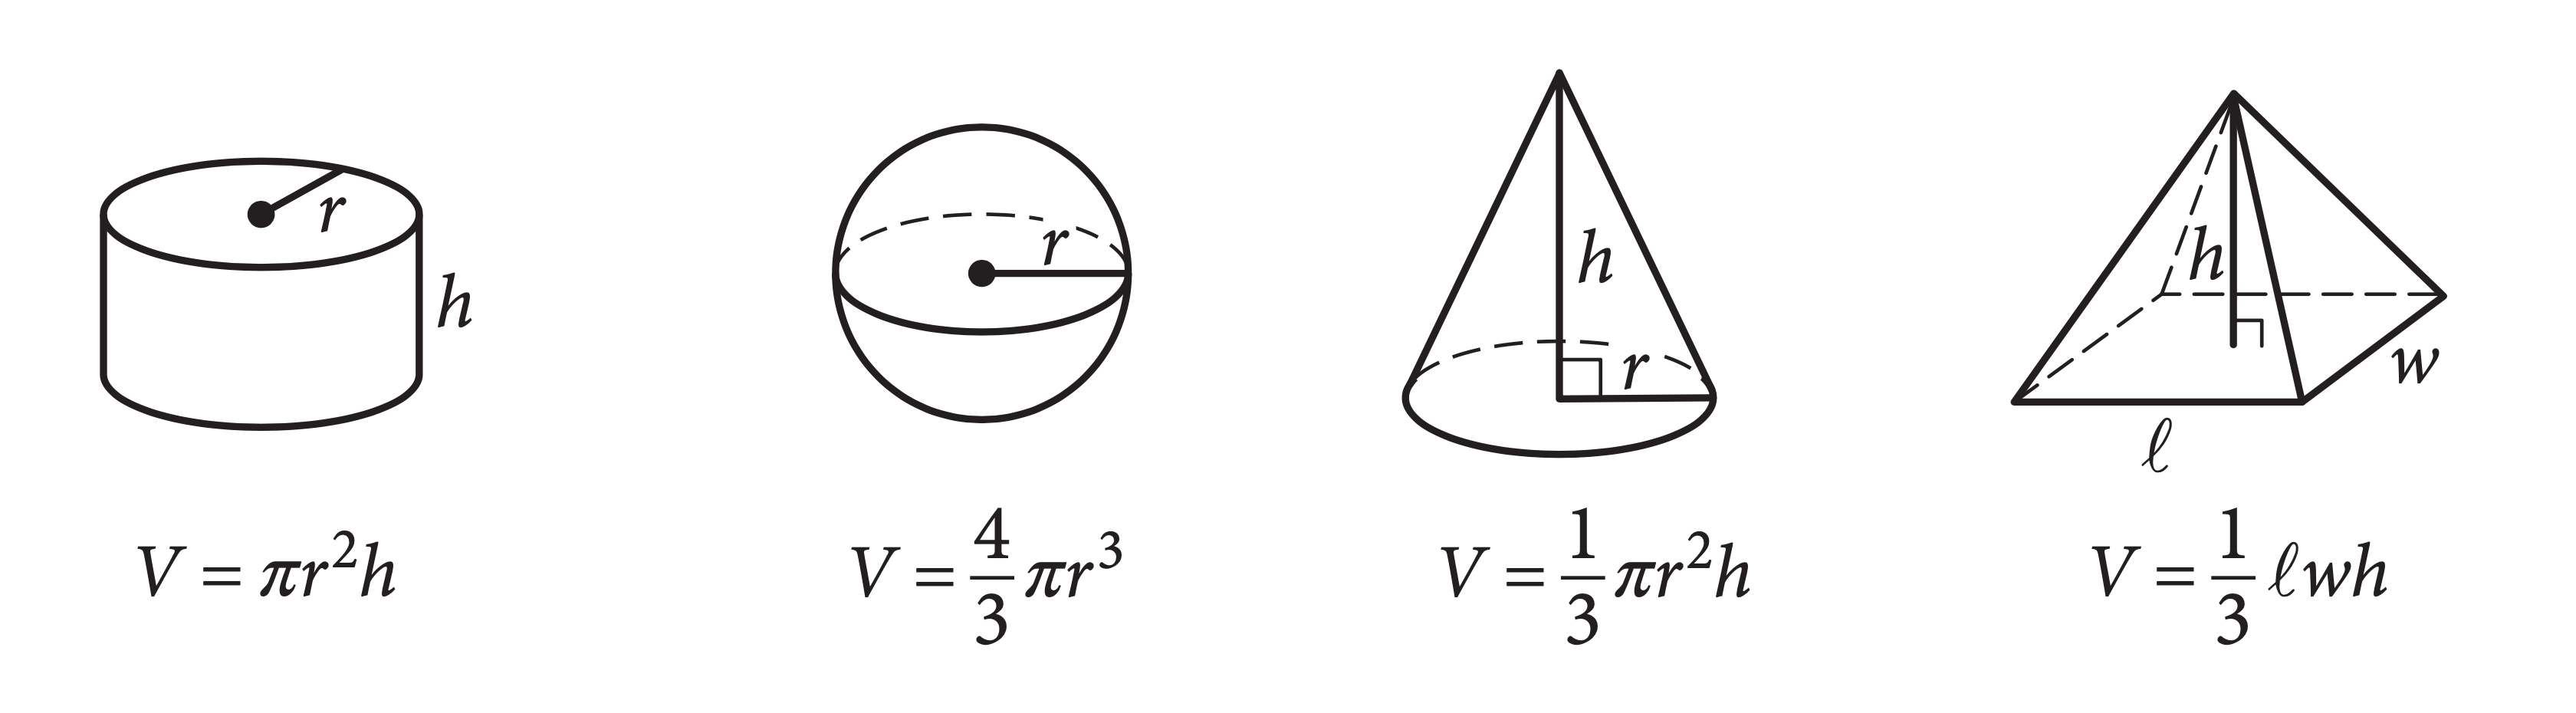
\includegraphics[width=150mm,scale=0.5]{SAT_Formulas.png}

}}\vspace{1mm}

\hspace{-1.2mm}
\noindent\fbox{\begin{minipage}[t][1.01\height][c]	{\dimexpr\textwidth-93.6\fboxsep-2\fboxrule\relax}
		\centering
		\textbf{Exponents/Roots/Logs}\vspace{2mm}\hline \\ \vspace{1.6mm}
		$2^{-2}=\tfrac{1}{4} \hspace{6mm} 2^{-1}=\tfrac{1}{2} \hspace{6mm} 2^{0}=\tfrac{1}{1} \hspace{6mm} 2^1=\tfrac{2}{1} \hspace{6mm} 2^2=\tfrac{4}{1}$
		\vspace{2mm}\\
		$\sqrt{a} \times \sqrt{b} = \sqrt{ab}$
		\vspace{3mm}\\
		$a=\sqrt[d]{b^c} \Rightarrow a=b^{c/d} \Rightarrow$ $\sqrt[c/d]{a}=b \Rightarrow \sqrt[c]{a^d}=b$ \vspace{3mm}\\
		$i^0=1 \hspace{7mm} i^1=i \hspace{7mm} i^2=-1 \hspace{7mm} i^3=-i$
			\vspace{4mm}\\
		
		\begin{array}{cccc}
   			$\tfrac{x^a}{x^b} =x^{a-b} $ & & & $x^a\times x^b = x^{a+b}$ \vspace{3mm}\\
			$($x$^a)^b = x^{ab}$ & & & $\ln(a)^r=r\ln(a)$  \vspace{3mm}\\
			$\ln(a)-\ln(b)=\ln\begin{pmatrix}\tfrac {a}{b}\end{pmatrix}$ & & & $\ln(a) + \ln(b) = \ln(ab)$ \vspace{3mm}\\
			$\ln(x) =  log_e(x)$ & & & $\log_a b = c \Rightarrow  a^c=b$  \vspace{3mm}\\
			$\log_x(x)=1$ & & & $\log_b(x)=\tfrac {\log_a(x)}{\log_a(b)}$
        \end{array}
        
        \vspace{1mm}
	\end{minipage}
}
\noindent\fbox{\begin{minipage}[t][1.107\height][c]{\dimexpr\textwidth-93.6\fboxsep-2\fboxrule\relax}
		\centering
		\vspace{-3.5mm}
		\textbf{Statistics}
		\vspace{3mm}\hline
		\begin{flushleft}
		\textit{Mean} - average\\
		\textit{Median} - middle value in a sorted list\\
		\textit{Mode} - most frequent\\
		\textit{Range} - difference between smallest and largest\\~\\
		
		\textit{Fundamental counting principle} - multiply odds together to find the chances of two occurrences happening at once. Eg: the odds getting two heads is $\tfrac {1}{2} \times \tfrac {1}{2} = \tfrac {1}{4}$.
		\end{flushleft}
		
		\vspace{1.7mm}
	\begin{tikzpicture}[scale=0.8]
	\draw (0,0) rectangle (5,.5);
	\draw[solid] (-2,.25) -- (0,.25);
	\draw[solid] (5,.25) -- (7,.25);
		
		\node at (0,-.35) {$25^{th}\%$};
		
		\node at (5,-.35) {$75^{th}\%$};
		
		\draw[solid] (2,0) -- (2,.5);
		\node at (2,-.35) {$median$};
		
		\draw[solid] (7,.1) -- (7,.4);
		\node at (7,-.35) {$max$};
		
		\draw[solid] (-2,.1) -- (-2,.4);
		\node at (-2,-.35) {$min$};
		
		\node at (2.5,1) {\textbf{Box and whisker plot}}\\
	\end{tikzpicture} \vspace{-1.1mm}
		
\end{minipage}}\\ \vspace{1mm}




\fbox{\parbox{\dimexpr\linewidth-2\fboxsep-2\fboxrule\relax}{\centering \textbf{Linear Equations}\vspace{2mm}\hline \vspace{1mm} \\ 
	\begin{array}{lll}
		\textit{Standard form:} $ Ax+By=C$ & & \textit{Midpoint formula:} $ M= \begin{pmatrix}\dfrac{x_1+x_2}{2}, \dfrac{y_1+y_2}{2}\end{pmatrix}$ \vspace{-2mm}\\
		\textit{Slope-Intercept form:} $ y=mx+b$\\ 
		\textit{Point-slope form:} $ y-y_1=m(x-x_1)$ & & \textit{Distance formula:} $ d = \sqrt{(x_2-x_1)^2+(y_2-y_1)^2}$
	\end{array}
}}
\vspace{1mm}

}}\\
\vspace{1mm}
\fbox{\parbox{\dimexpr\linewidth-2\fboxsep-2\fboxrule\relax}{\centering \textbf{Matrices}  \vspace{2mm}\hline \\~\\ 
	\\ \vspace{2mm}
	
	\textbf{determinants}
	$\begin{pmatrix}
		a&b\\
		c&d\\
	\end{pmatrix} \Rightarrow ad-bc$ \\ \vspace{2mm}
	
	
	\hline \vspace{2mm}

		\textbf{multiplication}
		$\begin{pmatrix}
			a&b&c\\
			d&e&f\\
		\end{pmatrix}\times \begin{pmatrix}
			h&j\\
			k&l\\
			m&n\\
		\end{pmatrix} = \begin{pmatrix}
			(ah) + (bk) + (cm) & (aj) + (bl) + (cn) \\
			(dh) + (ek) + (fm) & (dj) + (el) + (fn)
		\end{pmatrix}$
	
}}\\
\vspace{1mm}
\fbox{\parbox{\dimexpr\linewidth-2\fboxsep-2\fboxrule\relax}{\centering \textbf{Trigonometry}\vspace{2mm}\hline    \\~\\
	\noindent\fbox{\begin{minipage}[t][1.07\height][c]
	{\dimexpr\textwidth-100\fboxsep-2\fboxrule\relax}
	
		\centering \textbf{Basic properties of triangles}\\
	
		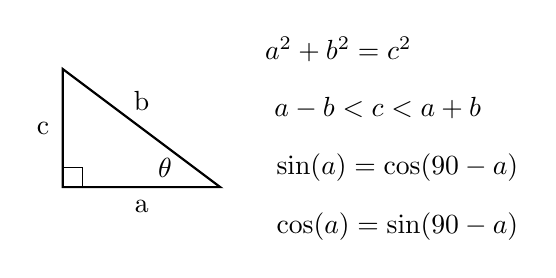
\begin{tikzpicture}
		\draw[thick]  (0,0)
		  -- (0,1.5) 
		  -- (2,0)
		  -- cycle;
		\draw (0,0) rectangle (.25,.25);
		\node at (1,-.25) {a};
		\node at (1,1.1) {b};
		\node at (-.25,.75) {c};
		\node at (1.3,.25) {$\theta$};
	
		\node at (3.5,1.75) {$a^2+b^2=c^2$};
		\node at (4,1) {$a-b < c < a+b$};
		\node at (4.25,.25) {$\sin(a) = \cos(90-a)$};
    	\node at (4.25,-.5) {$\cos(a) = \sin(90-a)$};
		
    	\end{tikzpicture}
    	
    	$\sin(\theta) =\tfrac {a}{c}$ \hfil $\cos(\theta) =\tfrac {b}{c}$ \hfil $\tan(\theta) =\tfrac {a}{b}$
    	
    	\vspace{-.9mm}
	\end{minipage}}
    \noindent\fbox{\begin{minipage}[t][1.03\height][c]
	{\dimexpr\textwidth-100\fboxsep-2\fboxrule\relax}
	
		\centering \textbf{Common values of trig functions}\\ \vspace{2mm}
	
		\renewcommand{\arraystretch}{1.6} \hspace{.5mm}
		\begin{tabular}{|c|c|c|c|c|c|c|}
    		\hline
    		\hspace{1mm} $\theta$ \hspace{1mm} & \hspace{1.5mm}$0$\hspace{1.5mm} &\hspace{1mm} $\tfrac {\pi}{6}$\hspace{2mm} &\hspace{1mm} $\tfrac {\pi}{4}$ \hspace{1mm} &\hspace{1mm} $\tfrac {\pi}{3}$ \hspace{1mm} & \hspace{1.5mm} $\tfrac {\pi}{2}$ \hspace{2mm} &\hspace{1mm} $\pi$\hspace{2mm} \\ \hline
    			$\sin \theta$ & $0$ & $\tfrac {1}{2}$ & $\tfrac {\sqrt{2}}{2}$ & $\tfrac {\sqrt{3}}{2}$ & $1$ & $0$\\ \hline
    			$\cos \theta$ & $1$ & $\tfrac {\sqrt{3}}{2}$ & $\tfrac {\sqrt{2}}{2}$ & $\tfrac {1}{2}$ & $0$ & $-1$ \\ \hline
    			$\tan \theta$ & $0$ & $\tfrac {\sqrt{3}}{3}$ & $1$ & $\sqrt{3}$ & $\infty$ & $0$ \\ \hline
    
    	\end{tabular}
    	\vspace{1mm}
	\end{minipage}} \\ \vspace{1mm}
	\noindent\fbox{\begin{minipage}[t][1.48\height][c]	{\dimexpr\textwidth-100\fboxsep-2\fboxrule\relax}
		\centering
		\textbf{Law of sines}\\ \vspace{2mm}
		$\dfrac {\sin (A) }{a} = \dfrac {\sin (B) }{b} = \dfrac {\sin (C) }{c}$
	\end{minipage}}
	\noindent\fbox{\begin{minipage}[t][1.2\height][c]{\dimexpr\textwidth-100\fboxsep-2\fboxrule\relax}
		\centering
		\textbf{Law of cosines}\\ \vspace{3.75mm}
		$a^2=b^2+c^2-2bc\cos(A)$ \vspace{1mm}
	\end{minipage}}\\ \vspace{1mm}

	\noindent\fbox{\begin{minipage}[t][1.12\height][c]	{\dimexpr\textwidth-100\fboxsep-2\fboxrule\relax}
		\centering
		\textbf{Simplifying trig functions}\\ \vspace{4mm}
		$\sin(a+b) = \sin(a)\cos(b)+\cos(a)\sin(b)$\vspace{1mm}
		$\cos(a+b) = \cos(a)\cos(b)-\sin(a)\sin(b)$\vspace{1mm}
		$\sin(a-b) = \sin(a)\cos(b)-\cos(a)\sin(b)$\vspace{1mm}
		$\cos(a-b) = \cos(a)\cos(b)+\sin(a)\sin(b)$\vspace{1mm}\vspace{1.5mm}
	\end{minipage}}
	\noindent\fbox{\begin{minipage}[t][1.12\height][c]{\dimexpr\textwidth-100\fboxsep-2\fboxrule\relax}
		\centering
		\textbf{Trig functions with the unit circle}\\ \vspace{2mm}
		$\begin{array}{ccccccc}
   		\sin(\theta) = \dfrac {y}{r} & & & \cos(\theta) = \dfrac {x}{r} & & & \tan(\theta) = \dfrac {y}{x} \vspace{5mm} \\ 
   		\csc(\theta) = \dfrac {r}{y} & & & \sec(\theta) = \dfrac {r}{x} & & & \cot(\theta) = \dfrac {x}{y}\\
    \end{array}$ \vspace{3mm} \\
    $x^2+y^2=r^2$
	\end{minipage}}\\ \vspace{1mm}
	
	\noindent\fbox{\begin{minipage}[t][1.1\height][c]	{\dimexpr\textwidth-100\fboxsep-2\fboxrule\relax}
		\centering
		\textbf{Reciprocal Identities}\\ \vspace{2mm}
		$\cot \theta = {{1}\over{\tan\theta}}$
		\hspace{8mm}
		$\sec \theta = {{1}\over{\cos\theta}}$
		\hspace{8mm}
		$\csc \theta = {{1}\over{\sin\theta}}$\\ \vspace{2mm}
	\end{minipage}}
	\noindent\fbox{\begin{minipage}[t][1.1\height][c]	{\dimexpr\textwidth-100\fboxsep-2\fboxrule\relax}
		\centering
		\textbf{Quotient Identities}\\ \vspace{2mm}
		$\tan \theta = {{\sin\theta}\over{\cos\theta}}$
		\hspace{10mm}
		$\cot \theta = {{\cos\theta}\over{\sin\theta}}$\\ \vspace{2mm}
	\end{minipage}}\\ \vspace{1mm}
	
	\noindent\fbox{\begin{minipage}[t][1.1\height][c]	{\dimexpr\textwidth-16\fboxsep-2\fboxrule\relax}
		\centering
		\textbf{Pythagorean Identities}\\ \vspace{2mm}
		$\sin ^{2}\theta+\cos ^{2}\theta=1$
		\hspace{10mm}
		$\tan ^{2}\theta+1=\sec ^{2}\theta$
		\hspace{10mm}
		$1+\cot ^{2}\theta=\csc ^{2}\theta$\\ \vspace{2mm}
	\end{minipage}}\\ \vspace{1mm}
	
	\hspace{.1mm} \noindent\fbox{\begin{minipage}[t][1.1\height][c]{\dimexpr\textwidth-80\fboxsep-2\fboxrule\relax}
		\centering \textbf{Double Angle Formulas}\\ \vspace{2mm}
		$\sin (2\theta) = 2\sin \theta \cos \theta \hspace{10mm}$
		$\cos (2\theta) = \cos^2\theta-\sin^2 \theta$
		\\ \vspace{2mm}
		$\cos (2\theta) = 1 - 2\sin^2\theta \hspace{10mm}$
		$\cos (2\theta) = 2\cos^2\theta -1$ \vspace{.1mm}

	\end{minipage}} 
	\noindent\fbox{\begin{minipage}[t][1.1\height][c]
		{\dimexpr\textwidth-120\fboxsep-2\fboxrule\relax}
	
		\centering \textbf{Heron's Formula}\\ \vspace{2mm}
	
		$\sqrt{s\cdot(s-a)(s-b)(s-c)}$\\ \vspace{1mm} 
		$s = \tfrac{a+b+c}{2}$\\ \vspace{.7mm}
	
	\end{minipage}} \vspace{1mm}
	
	\hspace{0mm} \noindent\fbox{\begin{minipage}[t][1.1\height][c]
	{\dimexpr\textwidth-100\fboxsep-2\fboxrule\relax}
	
	\centering \textbf{Calculating a triangle's area}\\ \vspace{2mm}
	
	area = $\dfrac {1}{2}ab\sin(C\degree)$ \vspace{1mm}
	
	\end{minipage}}
	\noindent\fbox{\begin{minipage}[t][1.1\height][c]
	{\dimexpr\textwidth-142\fboxsep-2\fboxrule\relax}
	
	\centering \textbf{Sector Arc Length}\\ \vspace{1mm}
	
	$s=r\theta$\\ where $\theta$ is in radians \vspace{1.5mm}
	
	\end{minipage}}
	\noindent\fbox{\begin{minipage}[t][1.4\height][c]
	{\dimexpr\textwidth-142\fboxsep-2\fboxrule\relax}
	
	\centering \textbf{Sector Area}\\ \vspace{3.45mm}
	
	$A=\dfrac {1}{2}\theta r^2$	
	\end{minipage}} \vspace{1mm}
	
	
	
	
    	
	\vspace{4mm}
}}


\vspace{1mm}
\fbox{\parbox{\dimexpr\linewidth-2\fboxsep-2\fboxrule\relax}{\centering \textbf{Calculus}  \vspace{2mm}\hline 
	\\~\\
	
	\textbf{Limits}
	\\
	
	If for every number $\epsilon > 0$ there is a number $\delta > 0$ such that if $0 < \abs{ x - a} < \delta$ then $\abs{ f(x) - L} < \epsilon.$
	
	\vspace{4mm}
	
	\begin{array}{cccc}
    $\textbf{Power Rule}$ & & & $\textbf{Quotient Rule}$ \\ \vspace{2mm}
    $\dfrac {d}{dx}[ax^n] = (n \times a)x^{n-1}$ & & & $\dfrac {d}{dx}\biggl[\dfrac {f(x)}{g(x)}\biggr] = \dfrac {g(x)f'(x)-f(x)g'(x)}{g(x)\times g(x)}$ \\
    $\textbf{Product Rule}$ & & & $\textbf{Chain Rule}$\\\vspace{2mm}
    $\dfrac {d}{dx}[f(x)g(x)] = f(x)g'(x)+f'(x)g(x)$ & & & $\dfrac {d}{dx}[f(g(x))] = f'(g(x)) \times g'(x)$  \\
    $\textbf{Exponential Rule}$ & & & $\textbf{Log Rule}$\\
    $\dfrac {d}{dx}[x^{a+b}] = x^{a+b} \times ln(x)(a+b)'$ & & & $\dfrac {d}{dx}[log_ax] = \dfrac {1}{x\times ln(a)} \times x'$
    \end{array}\\ \vspace{4.5mm}
    
    \textbf{Basic Derivatives}
    
    \vspace{1mm}
    
    \renewcommand{\arraystretch}{1.3}
    \begin{array}{cccc}
    	$\tfrac {d}{dx}(\sin x) = \cos x$ & $\tfrac {d}{dx}(-\sin x) = -\cos x$ & $\tfrac {d}{dx}(\cos x) = -\sin x$ & $\tfrac {d}{dx}(-\cos x) = \sin x$ \\
        	$\tfrac {d}{dx}(\sinh x) = \cosh x$ & $\tfrac {d}{dx}(-\sinh x) = -\cosh x$ & $\tfrac {d}{dx}(\cosh x) = \sinh x$ & $\tfrac {d}{dx}(-\cosh x) = -\sinh x$ \\
        $\tfrac {d}{dx}(\tan x) = \sec^2x$ & $\tfrac {d}{dx}(\cot x) = -\csc^2 x$ & $\tfrac {d}{dx}(\sec x) = \sec x \tan x$ & $\tfrac {d}{dx}(\csc x) = -\csc x \cot x$  \\
        $\tfrac {d}{dx}(\arcsin x) = \tfrac {1}{\sqrt{1-x^2}}$ &
        	$\tfrac {d}{dx}(\arccos x) = \tfrac {-1}{\sqrt{1-x^2}}$ & $\tfrac {d}{dx}(\arctan x) = \tfrac {1}{1+x^2}$ & $ f'(x) = \lim_{h\to 0 } \tfrac{f(x+h)-f(x)}{h}$
        	\\
        	$\tfrac {d}{dx}(e^{2x})=2e^x$ & $\tfrac {d}{dx}(a^{x})=a^{x}\ln a$ & $\tfrac {d}{dx}(\ln x)=\tfrac {1}{x}$ & $\tfrac {d}{dx}(\log_bx) = \tfrac{1}{x\ln(b)}$
    \end{array}\\         
    \vspace{.5mm}
    

    
    \noindent\fbox{\begin{minipage}[t][1.03\height][c]
	{\dimexpr\textwidth-128\fboxsep-2\fboxrule\relax}
	
		\centering \textbf{Position, velocity and acceleration}\\ \vspace{1.5mm}
		\hline
		\vspace{1.5mm}
		
		
		\textit{Position}\\ \vspace{1.5mm}
		\hspace{1mm} unit \Rightarrow $ x(t)$ \hspace{2.5mm}\\
		\hspace{-10.5mm} \tiny ex. \normalsize meters \Rightarrow $ x(t)$ \\ \vspace{1mm} \hline \vspace{1mm}
		
		\textit{Velocity}\\ \vspace{1.5mm}
		\hspace{1mm} \tfrac {unit}{time} \Rightarrow $ x'(t)$ \hspace{2.5mm}\\ \vspace{2mm}
		\hspace{-8.5mm} \tiny ex.\hspace{-2mm} \normalsize \tfrac {meters}{second} \Rightarrow $ v(t)$ \\ \vspace{2mm} \hline \vspace{1mm}
		
		\textit{Acceleration}\\ \vspace{1.5mm}
		\hspace{1mm} \tfrac {unit}{time^2} \Rightarrow $ x''(t)$ \hspace{2.5mm}\\ \vspace{2mm}
		\hspace{-9.5mm} \tiny ex.\hspace{-2mm} \normalsize \tfrac {meters}{second^2} \Rightarrow $ a(t)$ \\
				
		
    	\vspace{3.25mm}
	\end{minipage}} \hspace{-8pt}
	\arraycolsep=2pt\def\arraystretch{.75}
		\begin{array}[t]{@{}cc@{}}
			\noindent\fbox{\begin{minipage}[t][1.05\height][c]
			{\dimexpr\textwidth-128\fboxsep-2\fboxrule\relax}
	\centering \textbf{Rolle's Theorem}\\ 
	
			If $f(x)$ is continuous on $[a,b]$, differentiable on $(a,b)$ and $f(a)=f(b)=0$, then there exists a value for $c$ on the interval $(a,b)$ such that $f'(c)=0$.
			\vspace{1mm}
			\end{minipage}}
		&
			\noindent\fbox{\begin{minipage}[t][1.05\height][c]
			{\dimexpr\textwidth-128\fboxsep-2\fboxrule\relax}
	
			\centering \textbf{Intermediate Value Theorem}\\ \vspace{2mm}
	
			If $f(x)$ is continuous on $[a,b]$ and $c$ falls between $f(a)$ and $f(b)$, then there is at least one value of $x$ in which $f(x) = c$ on the interval $(a,b)$.
			
			\end{minipage}}
		&
			\noindent\fbox{\begin{minipage}[t][1.1\height][c]
			{\dimexpr\textwidth-128\fboxsep-2\fboxrule\relax}
			\centering \textbf{Mean Value Theorem}\\ \vspace{1mm}
	
			If $f(x)$ is continuous on $[a,b]$, differentiable on $(a,b)$ and $a<c<b$, then there exists a value for $c$ such that  \\ 
			$f'(c)=\tfrac {f(b)-f(a)}{b-a}$
			
			\end{minipage}}
		&
			\noindent\fbox{\begin{minipage}[t][1.05\height][c]
			{\dimexpr\textwidth-128\fboxsep-2\fboxrule\relax}
			\centering \textbf{Extreme Value Theorem}\\ \vspace{1mm}
	
			If $f(x)$ is continuous on $[a,b]$, then there exists both a minimum and a maximum on the interval $[a,b]$.
			\vspace{5.5mm}
			
			\end{minipage}} \\    
    \end{array} 
	\vspace{-.75mm}
	
	\vspace{1.5mm}
	\hspace{-2.75mm}
	\noindent\fbox{\begin{minipage}[t][1.45\height][c]
	{\dimexpr\textwidth-128\fboxsep-2\fboxrule\relax}
	
	\centering \textbf{Rewriting Riemann Sums}\\ \vspace{-5mm}
				
			\footnotesize
    		$$\lim_{n\to\infty} \sum_{k=1}^{n} f(x_x) \Delta x = \int_{a}^{b} f(x)dx$$


	
	\end{minipage}}
	\noindent\fbox{\begin{minipage}[t][1.1\height][c]
	{\dimexpr\textwidth-72\fboxsep-2\fboxrule\relax}
	
	\centering \textbf{Trapezoidal Sums}\\ \vspace{3mm}
				
		$\int_{a}^{b}f(x)dx\approx 
		\tfrac {1}{2}\tfrac {b-a}{n}[y_0+2y_1+2y_2...2y_{n-1}+2y_{n-1}+y_n]$
		\vspace{3mm}
	
	\end{minipage}}
	
	\vspace{1mm}
	\hspace{-2.75mm}
	\noindent\fbox{\begin{minipage}[t][1.3\height][c]
	{\dimexpr\textwidth-128\fboxsep-2\fboxrule\relax}
	
	\centering \textbf{Right Riemann Sums}\\ \vspace{2mm}
	
	\footnotesize $\tfrac {b-a}{n}[f(x_1)+f(x_2)...f(x_n)]$
	
	\end{minipage}}
	\noindent\fbox{\begin{minipage}[t][1.3\height][c]
	{\dimexpr\textwidth-128\fboxsep-2\fboxrule\relax}
	
	\centering \textbf{Left Riemann Sums}\\ \vspace{2mm}
	
	\footnotesize $\tfrac {b-a}{n}[f(x_0)+f(x_1)...f(x_{n-1})]$
		
	\end{minipage}}
	\noindent\fbox{\begin{minipage}[t][1.3\height][c]
	{\dimexpr\textwidth-128\fboxsep-2\fboxrule\relax}
	
	\centering \textbf{Midpoint Riemann Sums}\\ \vspace{2mm}
	
	\footnotesize $\tfrac {b-a}{n}[f(x_{1/2})+f(x_{3/2})...f(x_{n-1/2})]$
	
	\end{minipage}}

	\vspace{1mm}
	\hspace{-2.75mm}
	\noindent\fbox{\begin{minipage}[t][1.2\height][c]
	{\dimexpr\textwidth-128\fboxsep-2\fboxrule\relax}
	
	\centering \textbf{l'Hopital's Rule}\\ \vspace{1mm}
	
	If $\tfrac {f(a)}{g(b)}=\tfrac {0}{0}$ or $\tfrac {\infty}{\infty}$, then $\lim_{x\to a}\tfrac {f(x)}{g(x)}=\lim_{x\to a}\tfrac {f'(x)}{g'(x)}$
		
	\end{minipage}}
	\noindent\fbox{\begin{minipage}[t][1\height][c]
	{\dimexpr\textwidth-150\fboxsep-2\fboxrule\relax}
	
	\centering \textbf{Moebius strip}\\ \vspace{1mm}
	
	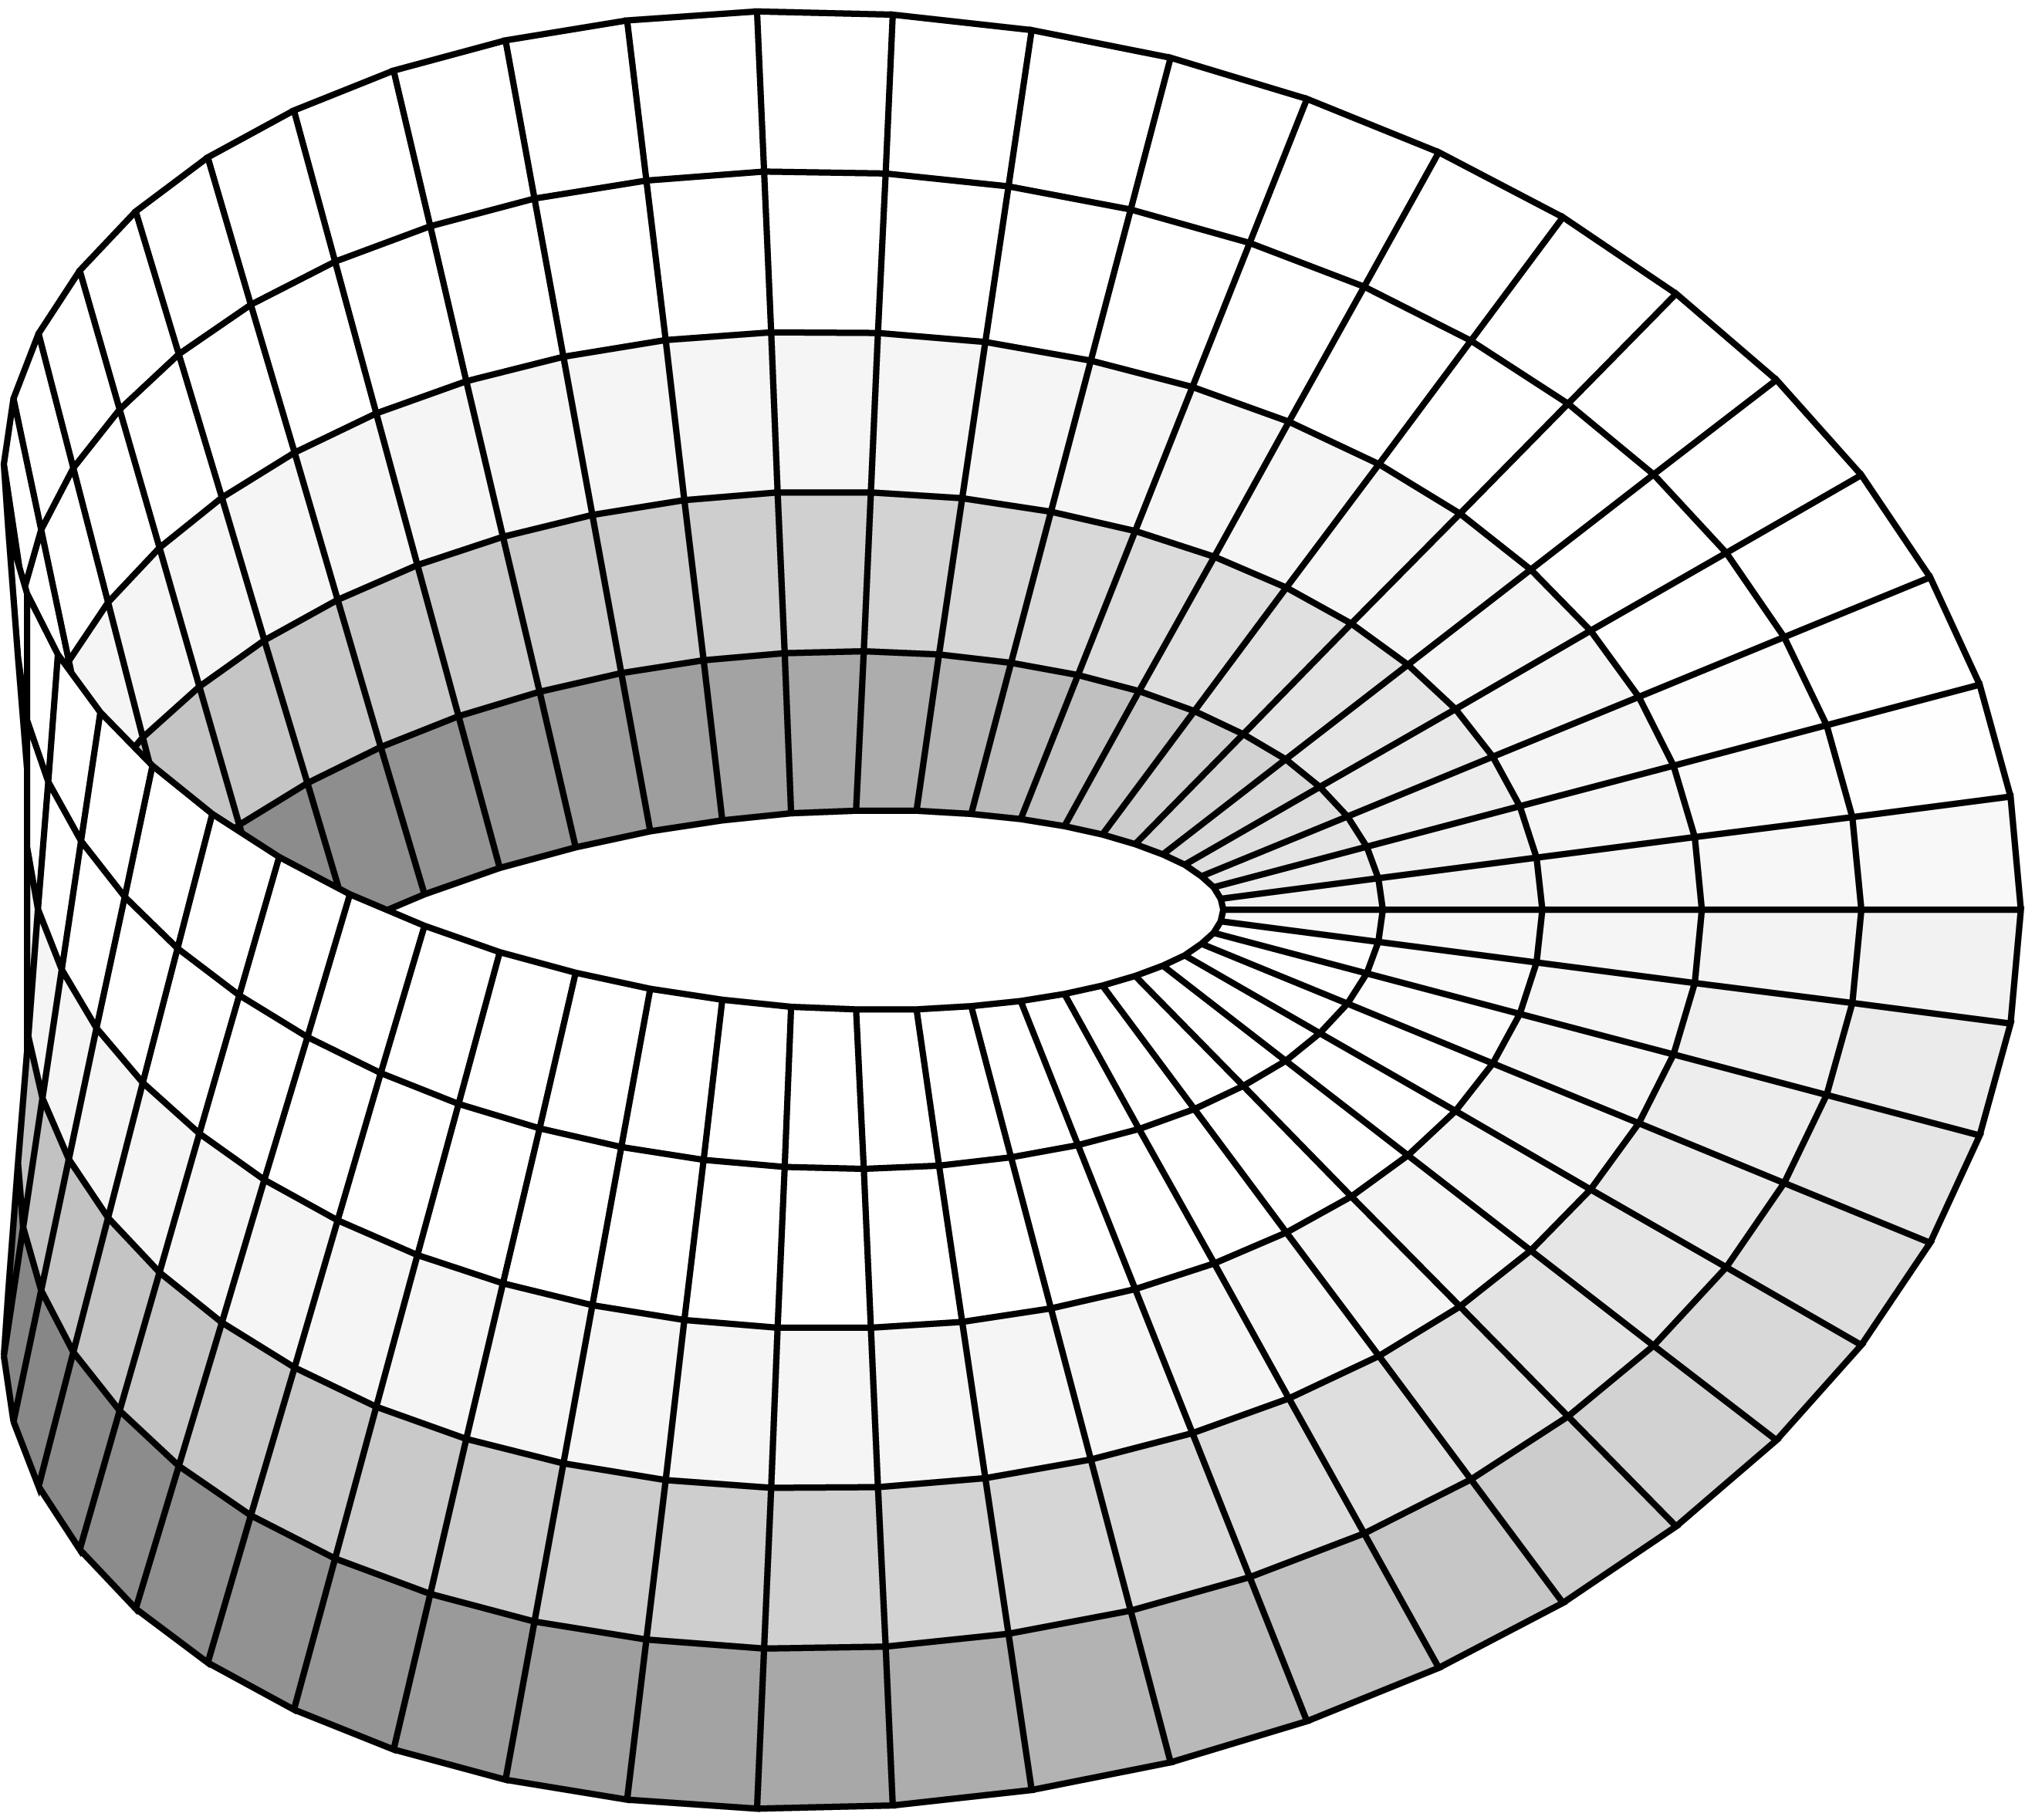
\includegraphics[width=15mm,scale=1]{moebius_strip.png}
	\vspace{.25mm}
		
	\end{minipage}}
	\noindent\fbox{\begin{minipage}[t][134\height][c]
	{\dimexpr\textwidth-106\fboxsep-2\fboxrule\relax}
		
		\hspace{-2.95mm}
		\renewcommand{\arraystretch}{1.35} 
		\begin{tabular}[t]{|c|c|c|c|c|c|c|}
    		\hline
    		$f(x)$  &\hspace{.25mm}+\hspace{.25mm} &\hspace{-.1mm} -\hspace{.92mm} & +m & -m &\footnotesize rel min &\footnotesize rel max \\ \hline
    		$f'(x)$ & & & + & - & +m & -m \\ \hline
    		$f''(x)$ & & & & & + & - \\ \hline
    	\end{tabular}
	\end{minipage}}
	
   	\vspace{2mm}

    
}}

\newpage

\vspace{1mm}

\fbox{\parbox{\dimexpr\linewidth-2\fboxsep-2\fboxrule\relax}{\centering \textbf{Constants}  \vspace{2mm}\hline 
	\\~\\
	$\pi \approx 3.14159$ \hfil
	$e\approx 2.71828$ \hfil
	$\gamma \approx 0.57721$ \hfil
	$\phi = {{1 + \sqrt 5 } \over 2} \approx 1.61803$ \hfil
	$\hat\phi = {{1 - \sqrt 5 } \over 2} \approx -.61803$ \hfil\end{minipage}
}}

\vspace{1mm}

\fbox{\parbox{\dimexpr\linewidth-2\fboxsep-2\fboxrule\relax}{\centering \textbf{Waves}  \vspace{2mm}\hline 
	\\~\\
	
	\noindent\fbox{\begin{minipage}[t][1.1\height][c]	{\dimexpr\textwidth-100\fboxsep-2\fboxrule\relax}
		\centering
		\textbf{Sine and cosine}\\ \vspace{2mm}
		$y=A\sin (Bx+C)+D$\\ 
		
	\begin{flushleft}
	\hspace{2mm}\textit{period:} $\dfrac {2\pi}{B}$ \hspace{15.5mm} \textit{amplitude:} $\abs{A}$\\ \vspace{1mm}
	\hspace{2mm}\textit{domain:} $ (-\infty ,\infty )$ \hspace{2mm} \textit{range:} $ [D-\abs{A}, D+\abs{A}]$\\ \vspace{1mm}
	\hspace{2mm}\textit{phase shift:} $ Bx + C = 0,$ \text{solve for $x$}\\ \vspace{1mm}
	\hspace{2mm}\textit{horizontal line of rest:} $ D$	\end{flushleft}
	
	\end{minipage}}
	\noindent\fbox{\begin{minipage}[t][1.1\height][c]	{\dimexpr\textwidth-100\fboxsep-2\fboxrule\relax}
		\centering
		\textbf{Cosecant and secant}\\ \vspace{2mm}
		$y=A\csc (Bx+C)+D$\\
		
	\begin{flushleft}
	\hspace{2mm}\textit{period:} $\dfrac {2\pi}{B}$ \hspace{5mm} \textit{amplitude:} $none$\\ \vspace{1mm}
	\hspace{2mm}\footnotesize \textit{domain:} $\csc \ne 0$ \hspace{0mm} \textit{range:} $ (-\infty,D-\abs{A}] \cup [D+\abs{A},\infty)$\\ \vspace{1mm} \normalsize
	\hspace{2mm}\textit{phase shift:} $ Bx + C = 0,$ \text{solve for $x$}\\ \vspace{1mm}
	\hspace{2mm}\textit{horizontal line of rest:} $ D$	\end{flushleft}
	\vspace{-4.9mm}
	
	\end{minipage}}
	\\ \vspace{3mm}
\end{minipage}
}}

\vspace{1mm}

\fbox{\parbox{\dimexpr\linewidth-2\fboxsep-2\fboxrule\relax}{\centering \textbf{Parabolas} \vspace{2mm}\hline  \\~\\
	\noindent\fbox{\begin{minipage}[t][1.1\height][c]{\dimexpr\textwidth-85\fboxsep-40\fboxrule\relax}
		\centering \textit{Standard form}: $ax^2+bx+c=0$\\
		\textit{Vertex form}: $y=a(x-h)^2+k$\\~\\
		\textit{Discriminant}: From standard form, $b^2-4ac$ \\
		\underline{No real solutions} when discriminant $< 0$  \\
		\underline{One real solution} when discriminant $= 0$ \\
		\underline{Two real solutions} when discriminant $> 0$ \\ \vspace{3.5mm}
	\end{minipage}} 
	\noindent\fbox{\begin{minipage}[t][.9\height][c]
		{\dimexpr\textwidth-110\fboxsep-2\fboxrule\relax}
		\centering
		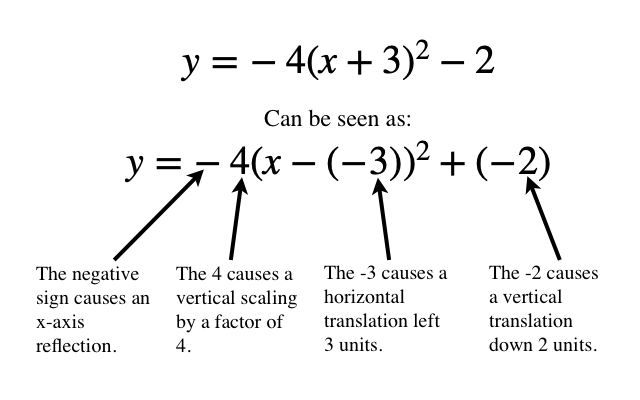
\includegraphics[width=75mm, scale=1]{parabola_form.png}
	\end{minipage}}\vspace{4mm}\\
	\textbf{Quadratic Formula:} $x=\dfrac{-b \pm \sqrt{b^2-4ac}}{2a}$
	\vspace{4mm}\\
}}

\vspace{1mm}

\noindent\fbox{\begin{minipage}[t][1.8\height][c]
	{\dimexpr\textwidth-133.5\fboxsep-2\fboxrule\relax}
	\centering
	\textbf{Units of Measurement}
	\vspace{1.75mm}\hline
	\vspace{2.15mm}
	
	\renewcommand{\arraystretch}{1.35} 
	\begin{array}{|c|c|} \hline
		$meter, m$ & $\footnotesize kilogram, kg$ \\ \hline
		$second, s$ & $ampere, A$ \\ \hline
		$kelvin, K$ & $mole, mol$ \\ \hline
		$mole, mol$ & $hertz, Hz$ \\ \hline
		$newton, N$ & $pascal, Pa$ \\ \hline
		$joule, J$ & $watt, W$ \\ \hline
		$coulomb, C$ & $volt, V$ \\ \hline
		$ohm, \Omega$ & $henry, H$ \\ \hline
		$farad, F$ & $tesla, T$  \\ \hline
    \end{array}\\
		
\end{minipage}}
\noindent\fbox{\begin{minipage}[t][1.8\height][c]
	{\dimexpr\textwidth-133.5\fboxsep-2\fboxrule\relax}
	\centering
	\textbf{Unit Prefixes}
	\vspace{1.75mm}\hline
	\vspace{2.15mm}
	
	\renewcommand{\arraystretch}{1.35} 
	\begin{array}{|c|c|c|} \hline
		$Prefix$ & $Symbol$ & $Factor$ \\ \hline
		$\textit{giga}$ & $\textit{G}$ & $10^9$ \\ \hline
		$\textit{mega}$ & $\textit{M}$ & $10^6$ \\ \hline
		$\textit{kilo}$ & $\textit{k}$ & $10^3$ \\ \hline
		$\textit{centi}$ & $\textit{c}$ & $10^{-2}$ \\ \hline
		$\textit{milli}$ & $\textit{m}$ & $10^{-3}$ \\ \hline
		$\textit{micro}$ & $\mu$ & $10^{-6}$ \\ \hline
		$\textit{nano}$ & $\textit{n}$ & $10^{-9}$ \\ \hline
		$\textit{pico}$ & $\textit{p}$ & $10^{-12}$ \\ \hline
    \end{array}\\
		
\end{minipage}}
\noindent\fbox{\begin{minipage}[t][1.005\height][c]	{\dimexpr\textwidth-103\fboxsep-2\fboxrule\relax}
		\centering
		\textbf{Pascal's Triangle}
		\vspace{1.25mm}\hline
		\vspace{1mm}
		1\\
		1 1\\
		1 2 1\\
		1 3 3 1\\
		1 4 6 4 1\\
		1 5 10 10 5 1\\
		1 6 15 20 15 6 1\\
		1 7 21 35 35 21 7 1\\
		1 8 28 56 70 56 28 8 1\\
		1 9 36 84 126 126 84 36 9 1\\
		1 10 45 120 210 252 210 120 41 10 1\\
		1 11 55 165 330 462 462 330 165 55 11 1\\
		1 12 66 220 495 792 924 792 495 220 66 12 1\\
		\vspace{1mm}
\end{minipage}}\\ 

\vspace{1mm}

\newpage

\end{center}

\end{document}